\documentclass{article}

\usepackage{amsmath}
\usepackage{geometry}
\usepackage{graphicx}

\usepackage[utf8]{inputenc}
\usepackage{fourier} 
\usepackage{array}
\usepackage{makecell}

\geometry{letterpaper, left=1cm, right=1cm, top=1.5cm, bottom=2cm}

\title{Translation Invariance Experiment}
\author{Adam Spindler}

\begin{document}
\maketitle

\section{Methodology}


The standard approach for creating adversarial images is to iteratively update an image so that the loss of the target model increases. The image is updated by computing the derivative of the loss function with respect to the input image, which gives you a tensor that points in the direction of increasing the loss function. This gradient is multiplied by a small constant (like 0.01) and added to the input image to slightly move it in the direction of increasing loss. This process is repeated iteratively until the image is modified enough to cause a mis-detection. For my experiments, I go several iterations beyond that to improve transferability.

In another attempt to increase the transferability of my adversarial examples I implemented the translation invariance technique as described in \cite{dong2019evading}. The idea behind this approach is to shift the adversarial image during its creation so that the adversarial image could be shifted after creation and still retain its adversarialness. This was also shown to increase transferability between models in their paper.

The way that this works specifically is that each iteration of the adversarial image creation, several copies of the current version of the image are made where each one is translated by a small amount. Then each image is passed through the model and its gradient is computed for the loss function. Each of these gradients are then translated back to where they would be on the original input image and averaged together. This combined gradient is then added to the input image. A graphical representation is illustrated in figure \ref{fig:translationInvariance}, and this idea is expressed mathematically below:
\vspace{0.5cm}

Original:
\begin{equation}
    X := X + \epsilon \nabla_X f_\text{ensemble}(X) 
\end{equation}

With Translation Invariance:
\begin{equation}
    X := X + \epsilon \frac{1}{N} \sum_{i = 1}^{N} T_i^{-1}(\nabla_X f_\text{ensemble}(T_i(X)))
\end{equation}

Where:
\vspace{0.5cm}

\begin{tabular}{l l}
    $X$ & Current version of input image \\
    $\epsilon$ & Learning Rate \\
    $f_{\text{ensemble}}$ & Ensemble of models which outputs a scalar loss, which is basically the sum of confidence scores \\
    $N$ & Number of translations \\
    $T$ & Translation function \\
    $T^{-1}$ & Inverse of translation function \\[1cm]
\end{tabular}

\begin{figure}
\centering
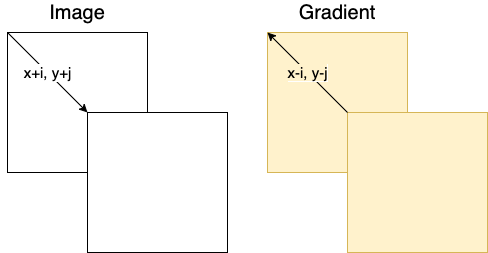
\includegraphics[width=0.5\linewidth]{images/translation-invariance.png}
\caption{The image is translated in the X and Y directions, shifting it before being passed into the network. Then the gradient is computed and shifted back to align its values with the original image.}
\label{fig:translationInvariance}
\end{figure}

For this experiment the following set of translations were used each iteration:

\begin{verbatim}
    [(0, 0), (2, 2), (4, 0), (0, 4), (-4, -4), (-8, 0), (0, -8), (0, 8), (0, 8), (8, 8), (-8, -8)]
\end{verbatim}

\begin{figure}
\begin{tabular}{c c c}
    Original & Ensemble Adversarial & Translation Invariant Ensemble Adversarial \\
    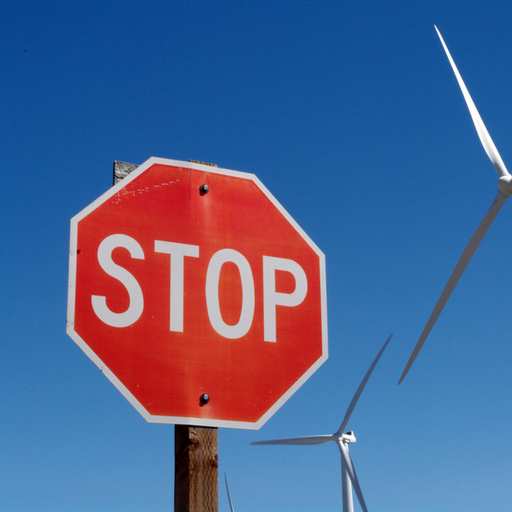
\includegraphics[width=0.3\linewidth]{../test_images/test_set20/431d3546f1189614.jpg} & 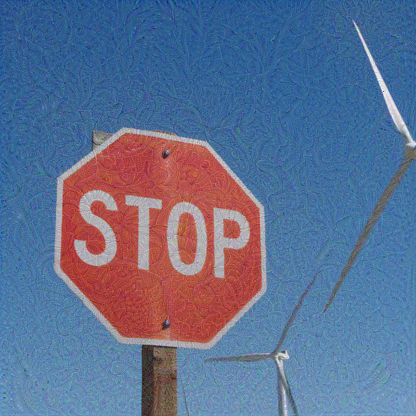
\includegraphics[width=0.3\linewidth]{../test_images/not_translated/ensemble_adversarial_431d3546f1189614.png}  & 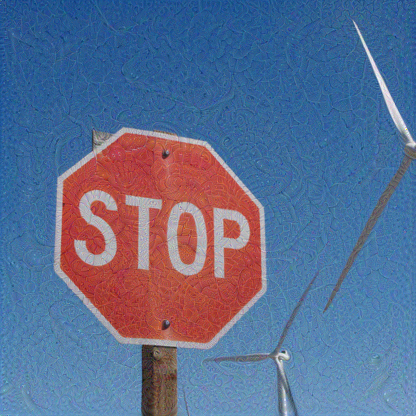
\includegraphics[width=0.3\linewidth]{../test_images/ensemble_translated/ensemble_adversarial_431d3546f1189614.png} \\
\end{tabular}
\caption{Visual Comparison of Adversarial Image Techniques}
\end{figure}

\subsection{Evaluation on AWS Rekognition}

20 images of stop signs were used to evaluate the effectiveness of this technique. These images are available in my GitHub repository in the "/test\_images/test\_set20/" directory. 3 sets of images were sent to AWS Rekognition for evaluation: the unmodified images, the regular ensemble adversarial images, and the translation invariant ensemble adversarial images. The results of this are listed in figure \ref{fig:awsEval}.

\begin{figure}
\centering
\begin{tabular}{l c c c}
    & \textbf{Original} & \textbf{Ensemble Adversarial} & \textbf{Translation Invariant Ensemble Adversarial} \\
    \textbf{Stop Sign} & \makecell{9 images \\ 78.497 avg confidence \\ 0 bboxes} & \makecell{15 images \\ 74.891 avg confidence \\ 0 bboxes} & \makecell{15 images \\ 71.905 avg confidence \\ 0 bboxes} \\[1cm]
    \textbf{Road Sign} & \makecell{18 images \\ 95.671 avg confidence \\ 24 bboxes} & \makecell{18 images \\ 91.348 avg confidence \\ 9 bboxes} & \makecell{18 images \\ 87.795 avg confidence \\ 5 bboxes} \\[1cm]
    \textbf{Sign} & \makecell{16 images \\ 96.117 avg confidence \\ 0 bboxes} & \makecell{19 images \\ 90.422 avg confidence \\ 0 bboxes} & \makecell{19 images \\ 88.508 avg confidence \\ 0 bboxes} \\[1cm]
\end{tabular}
\caption{The evaluation of adversarial images on AWS Rekognition, listing the number of images each class appeared in, the average confidence score of the detections, and the number of bounding boxes detected across all 20 images.}
\label{fig:awsEval}
\end{figure}

The confidence score of each of the classes did go down with this technique and so did the number of bounding boxes detected, at least for the "Road Sign" class. However, when creating the adversarial images in general it increased the number of images in which the stop signs and regular signs were detected which is unexpected.

Overall, this result is interesting though because there is a non-negligible decrease in the confidence score despite the translation invariant images looking very similar to the regular adversarial images I created. It also shows that translation invariance is effective at increasing transferability of adversarial images.

\section{Future Work}

The adversarial images created for this experiment have a moderate level of distortion applied. The images have clearly been altered, but they are easily detectable as a stop sign when looking at the images as a human. Each of these images were run for 30 iterations of adversarial updates which may not be enough to fool AWS. More significant alterations may be required to create transferable adversarial images.

In short, the things I can try next are: increase the number of iterations, increase the number of translations, and randomize which translations are used each iteration. I can also try limiting the image modifications to the inside of the bounding boxes of the stop signs.

\clearpage
\bibliographystyle{unsrt}
\bibliography{references}

\end{document}